\documentclass[../mathNotesPreamble]{subfiles}

\providecommand{\relscalefact}{1.4}
\begin{document}
\relscale{\relscalefact}
  \section{1.5: Transformation of Functions}
  %Vertical and horizontal shifts
  \begin{defn*}[Vertical Shift]
    Given a function $f(x)$, a new function $g(x)=f(x)+k$, where $k$ is a constant, is a \textbf{vertical shift} of the function $f(x)$. All the output values shift vertically by $k$ units (\textbf{up} if $h>0$, \textbf{down} if $h<0$).
  \end{defn*}
  \begin{ex*}
    Using the graphs below, sketch the shifted functions as indicated:
    \begin{extasks}[after-item-skip=\stretch{1}](2)
      \task
        Graph $f(x)+2$:

        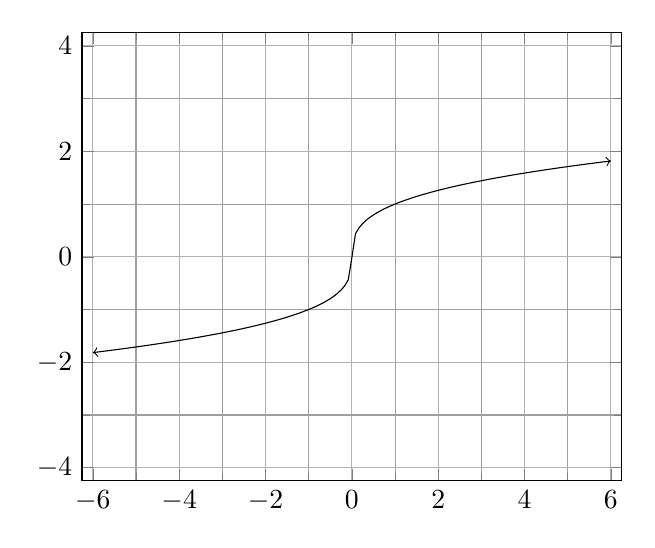
\begin{tikzpicture}[declare function={
          cubeRoot(\x)=\x/abs(\x)*abs(\x)^(1/3);}
          ]
          \begin{axis}[
            grid=both, %major,minor
            grid style={line width=0.375pt, draw=gray!60},
            minor grid style={draw=gray!75},
            xmin=-6.25, xmax=6.25,
            ymin=-4.25, ymax=4.25,
            minor x tick num=1,
            minor y tick num=1,
            ]
            \addplot[<-] expression[domain=-6:-1]{cubeRoot(x)};
            \addplot[-] expression[domain=-1:1]{cubeRoot(x)};
            \addplot[->] expression[domain=1:6]{cubeRoot(x)};
          \end{axis}
        \end{tikzpicture}
      \task
        Graph $f(x)-1$:

        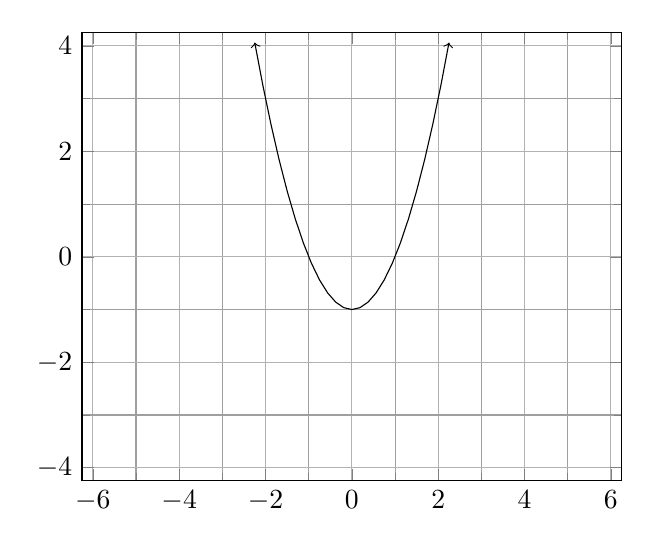
\begin{tikzpicture}[declare function={
          f(\x)=(\x-1)*(\x+1);}
          ]
          \begin{axis}[
            grid=both, %major,minor
            grid style={line width=0.375pt, draw=gray!60},
            minor grid style={draw=gray!75},
            xmin=-6.25, xmax=6.25,
            ymin=-4.25, ymax=4.25,
            minor x tick num=1,
            minor y tick num=1,
            ]
            \addplot[<->] expression[domain=-2.25:2.25]{f(x)};
          \end{axis}
        \end{tikzpicture}
    \end{extasks}
    \vspace*{\stretch{1}}
  \end{ex*}
  \pagebreak

  \begin{defn*}[Horizontal Shift]
    Given a function $f(x)$, a new function $g(x)=f(x-h)$, where $h$ is a constant, is a \textbf{horizontal shift} of the function $f(x)$. All the output values shift horizontally by $h$ units (\textbf{right} if $k>0$, \textbf{left} if $k<0$).
  \end{defn*}
  \begin{ex*}
    Using the graphs below, sketch the shifted functions as indicated:
    \begin{extasks}[after-item-skip=\stretch{1}](2)
      \task
        Graph $f(x+2)$:

        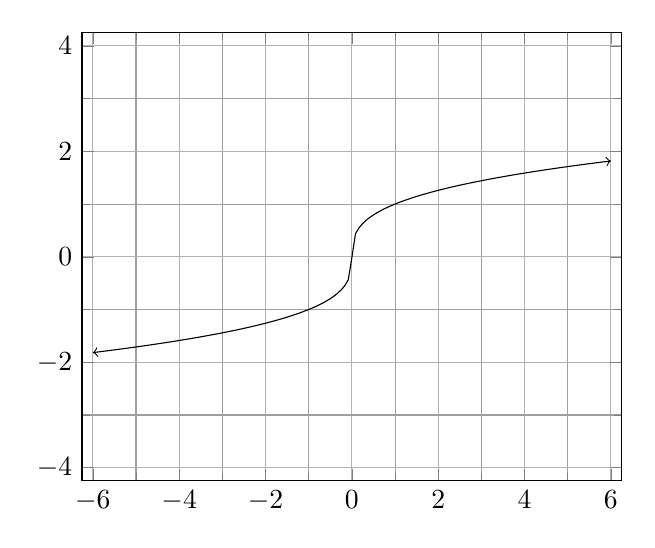
\begin{tikzpicture}[declare function={
          cubeRoot(\x)=\x/abs(\x)*abs(\x)^(1/3);}
          ]
          \begin{axis}[
            grid=both, %major,minor
            grid style={line width=0.375pt, draw=gray!60},
            minor grid style={draw=gray!75},
            xmin=-6.25, xmax=6.25,
            ymin=-4.25, ymax=4.25,
            minor x tick num=1,
            minor y tick num=1,
            ]
            \addplot[<-] expression[domain=-6:-1]{cubeRoot(x)};
            \addplot[-] expression[domain=-1:1]{cubeRoot(x)};
            \addplot[->] expression[domain=1:6]{cubeRoot(x)};
          \end{axis}
        \end{tikzpicture}

      \task
        Graph $f(x-1)$:

        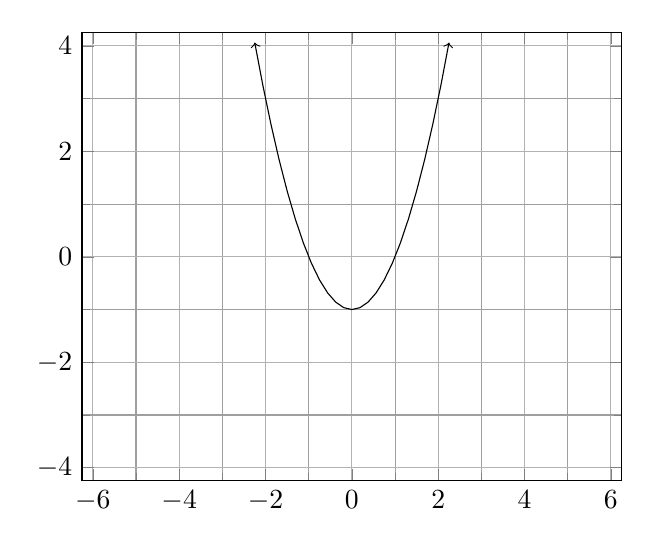
\begin{tikzpicture}[declare function={
          f(\x)=(\x-1)*(\x+1);}
          ]
          \begin{axis}[
            grid=both, %major,minor
            grid style={line width=0.375pt, draw=gray!60},
            minor grid style={draw=gray!75},
            xmin=-6.25, xmax=6.25,
            ymin=-4.25, ymax=4.25,
            minor x tick num=1,
            minor y tick num=1,
            ]
            \addplot[<->] expression[domain=-2.25:2.25]{f(x)};
          \end{axis}
        \end{tikzpicture}

      \task
        Graph $f(x-2)+1$:

        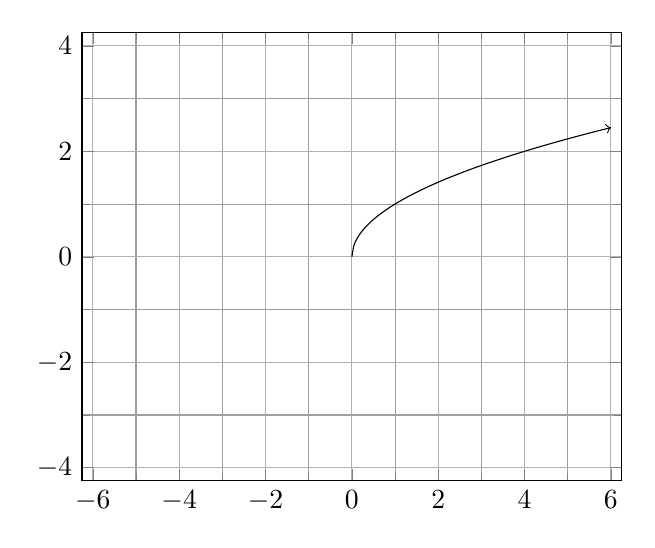
\begin{tikzpicture}
          \begin{axis}[
            grid=both, %major,minor
            grid style={line width=0.375pt, draw=gray!60},
            minor grid style={draw=gray!75},
            xmin=-6.25, xmax=6.25,
            ymin=-4.25, ymax=4.25,
            minor x tick num=1,
            minor y tick num=1,
            ]
            \addplot[-] expression[domain=0:1]{sqrt(x)};
            \addplot[->] expression[domain=1:6]{sqrt(x)};
          \end{axis}
        \end{tikzpicture}

      \task
        Graph $f(x+1)-3$:

        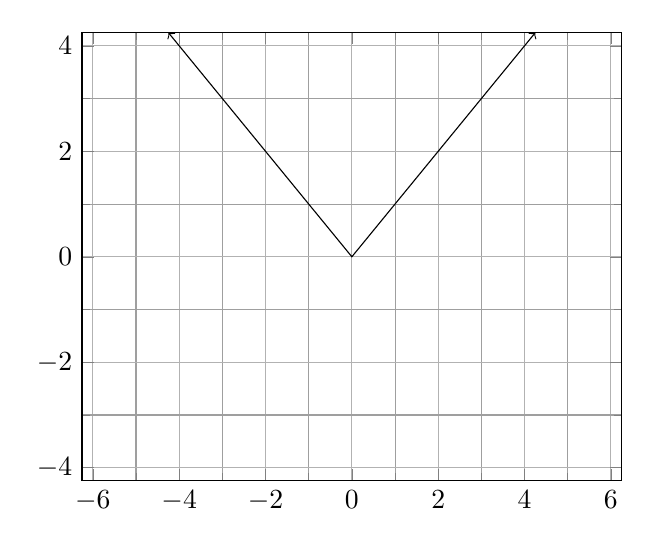
\begin{tikzpicture}
          \begin{axis}[
            grid=both, %major,minor
            grid style={line width=0.375pt, draw=gray!60},
            minor grid style={draw=gray!75},
            xmin=-6.25, xmax=6.25,
            ymin=-4.25, ymax=4.25,
            minor x tick num=1,
            minor y tick num=1,
            ]
            \addplot[<->] expression[domain=-4.25:4.25]{abs(x)};
          \end{axis}
        \end{tikzpicture}
    \end{extasks}
  \end{ex*}
  \pagebreak

  \begin{ex*}
    Identify the shifts which transform the blue graph into the red graph:
    \begin{extasks}[after-item-skip=\stretch{1}](2)
      \task
        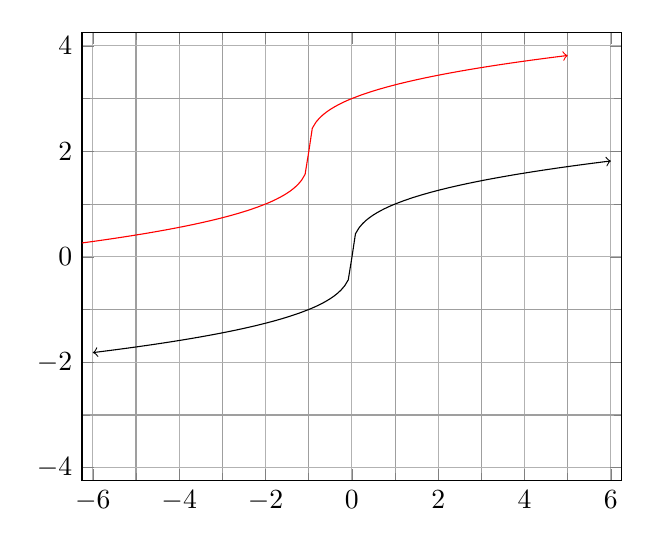
\begin{tikzpicture}[declare function={
          cubeRoot(\x)=\x/abs(\x)*abs(\x)^(1/3);
          h=-1; k=2;
          f(\x)=cubeRoot(\x-h)+k;}
          ]
          \begin{axis}[
            grid=both, %major,minor
            grid style={line width=0.375pt, draw=gray!60},
            minor grid style={draw=gray!75},
            xmin=-6.25, xmax=6.25,
            ymin=-4.25, ymax=4.25,
            minor x tick num=1,
            minor y tick num=1,
            ]

            \addplot[<-] expression[domain=-6:-1]{cubeRoot(x)};
            \addplot[-] expression[domain=-1:1]{cubeRoot(x)};
            \addplot[->] expression[domain=1:6]{cubeRoot(x)};
            %
            \addplot[<-, red] expression[domain=-6+h:-1+h]{f(x)};
            \addplot[-, red] expression[domain=-1+h:1+h]{f(x)};
            \addplot[->, red] expression[domain=1+h:6+h]{f(x)};
          \end{axis}
        \end{tikzpicture}

      \task
        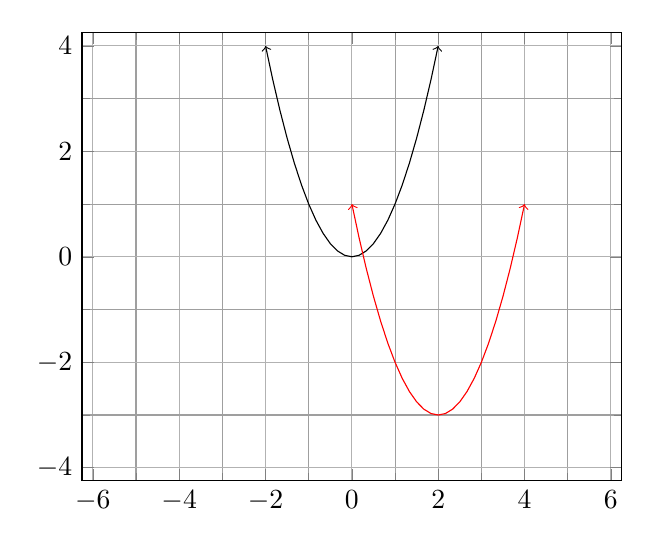
\begin{tikzpicture}[declare function={
          f(\x)=\x^2;
          h=2; k=-3;
          g(\x)=f(\x-h)+k;}
          ]
          \begin{axis}[
            grid=both, %major,minor
            grid style={line width=0.375pt, draw=gray!60},
            minor grid style={draw=gray!75},
            xmin=-6.25, xmax=6.25,
            ymin=-4.25, ymax=4.25,
            minor x tick num=1,
            minor y tick num=1,
            ]
            \addplot[<->] expression[domain=-2:2]{f(x)};
            %
            \addplot[<->, red] expression[domain=-2+h:2+h]{g(x)};
          \end{axis}
        \end{tikzpicture}

      \task
        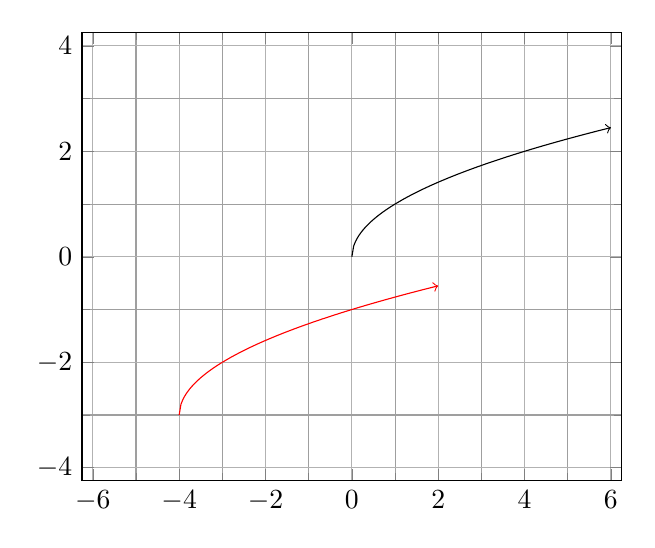
\begin{tikzpicture}[declare function={
          f(\x)=sqrt(\x);
          h=-4; k=-3;
          g(\x)=f(\x-h)+k;}]
          \begin{axis}[
            grid=both, %major,minor
            grid style={line width=0.375pt, draw=gray!60},
            minor grid style={draw=gray!75},
            xmin=-6.25, xmax=6.25,
            ymin=-4.25, ymax=4.25,
            minor x tick num=1,
            minor y tick num=1,
            ]
            \addplot[-] expression[domain=0:1]{f(x)};
            \addplot[->] expression[domain=1:6]{f(x)};
            %
            \addplot[-, red] expression[domain=0+h:1+h]{g(x)};
            \addplot[->, red] expression[domain=1+h:6+h]{g(x)};
          \end{axis}
        \end{tikzpicture}

      \task
        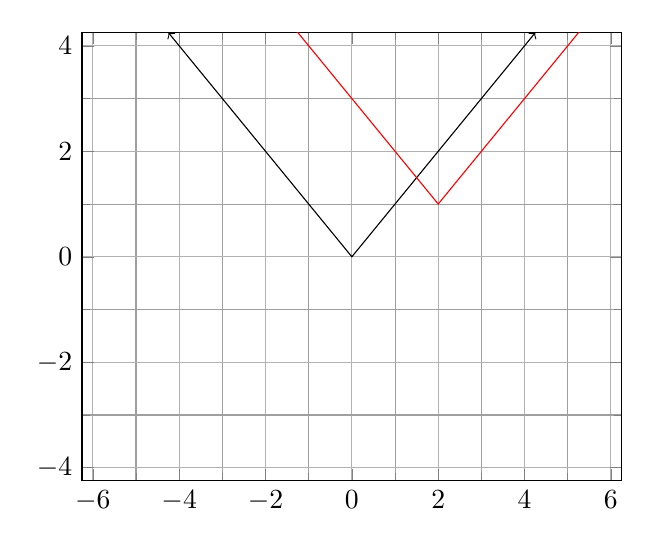
\begin{tikzpicture}[declare function={
          f(\x)=abs(\x);
          h=2; k=1;
          g(\x)=f(\x-h)+k;}]
          \begin{axis}[
            grid=both, %major,minor
            grid style={line width=0.375pt, draw=gray!60},
            minor grid style={draw=gray!75},
            xmin=-6.25, xmax=6.25,
            ymin=-4.25, ymax=4.25,
            minor x tick num=1,
            minor y tick num=1,
            ]
            \addplot[<->] expression[domain=-4.25:4.25]{f(x)};
            %
            \addplot[<->, red] expression[domain=-4.25+h:4.25+h]{g(x)};
          \end{axis}
        \end{tikzpicture}
    \end{extasks}
    \vspace*{\stretch{1}}
  \end{ex*}
  \pagebreak

  %Reflections about axes
  \begin{defn*}[Reflections]
    Given a function $f(x)$, a new function $g(x)=-f(x)$ is a \textbf{vertical reflection} of the function $f(x)$, sometimes called a reflection about the $x$-axis.
    \vspace*{0.5\baselineskip}

    Given a function $f(x)$, a new function $g(x)=f(-x)$ is a \textbf{horizontal reflection} of the function $f(x)$, sometimes called a reflection about the $y$-axis.
  \end{defn*}


  \begin{ex*}
    Transform the graphs below as indicated:
    \begin{extasks}[after-item-skip=\stretch{1}](2)
      \task
        Graph $f(-x)$:

        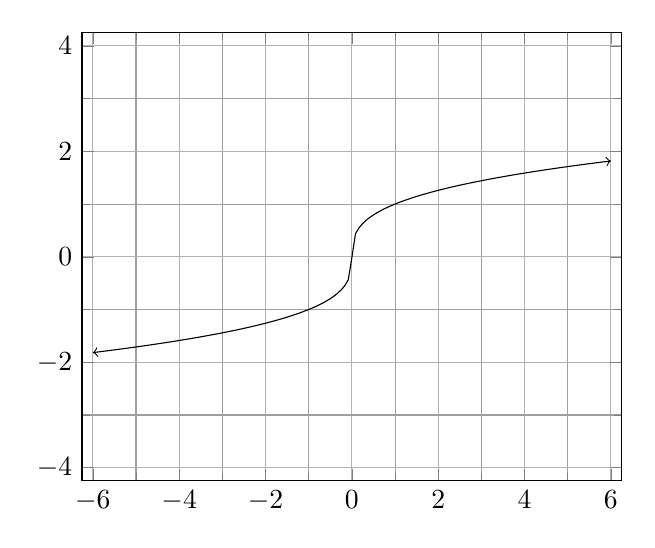
\begin{tikzpicture}[declare function={
          cubeRoot(\x)=\x/abs(\x)*abs(\x)^(1/3);}]
          \begin{axis}[
            grid=both, %major,minor
            grid style={line width=0.375pt, draw=gray!60},
            minor grid style={draw=gray!75},
            xmin=-6.25, xmax=6.25,
            ymin=-4.25, ymax=4.25,
            minor x tick num=1,
            minor y tick num=1,
            ]
            \addplot[<-] expression[domain=-6:-1]{cubeRoot(x)};
            \addplot[-] expression[domain=-1:1]{cubeRoot(x)};
            \addplot[->] expression[domain=1:6]{cubeRoot(x)};
          \end{axis}
        \end{tikzpicture}

      \task
        Graph $-f(x)$:

        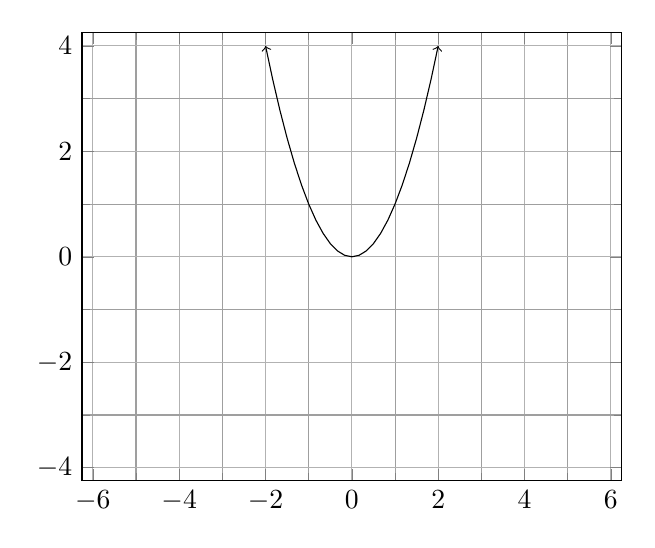
\begin{tikzpicture}[declare function={
          f(\x)=\x^2;}]
          \begin{axis}[
            grid=both, %major,minor
            grid style={line width=0.375pt, draw=gray!60},
            minor grid style={draw=gray!75},
            xmin=-6.25, xmax=6.25,
            ymin=-4.25, ymax=4.25,
            minor x tick num=1,
            minor y tick num=1,
            ]
            \addplot[<->] expression[domain=-2:2]{f(x)};
          \end{axis}
        \end{tikzpicture}

      \task
        Graph $-f(-x)$:

        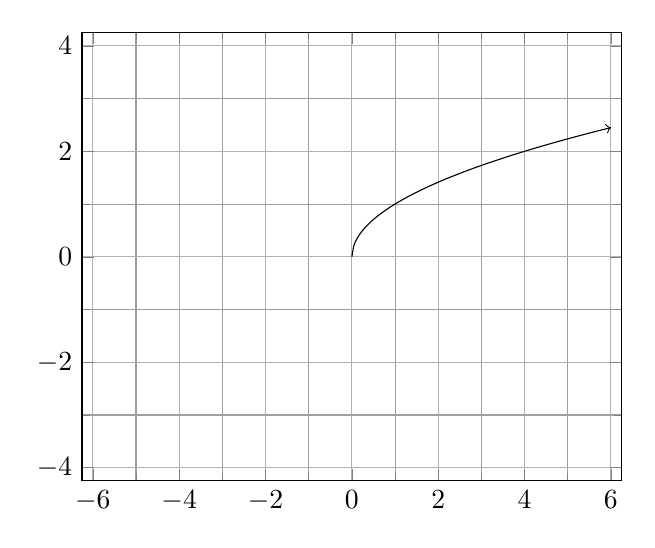
\begin{tikzpicture}[declare function={
          f(\x)=sqrt(\x);}]
          \begin{axis}[
            grid=both, %major,minor
            grid style={line width=0.375pt, draw=gray!60},
            minor grid style={draw=gray!75},
            xmin=-6.25, xmax=6.25,
            ymin=-4.25, ymax=4.25,
            minor x tick num=1,
            minor y tick num=1,
            ]
            \addplot[-] expression[domain=0:1]{f(x)};
            \addplot[->] expression[domain=1:6]{f(x)};
          \end{axis}
        \end{tikzpicture}

      \task
        Graph $-f(x)+1$

        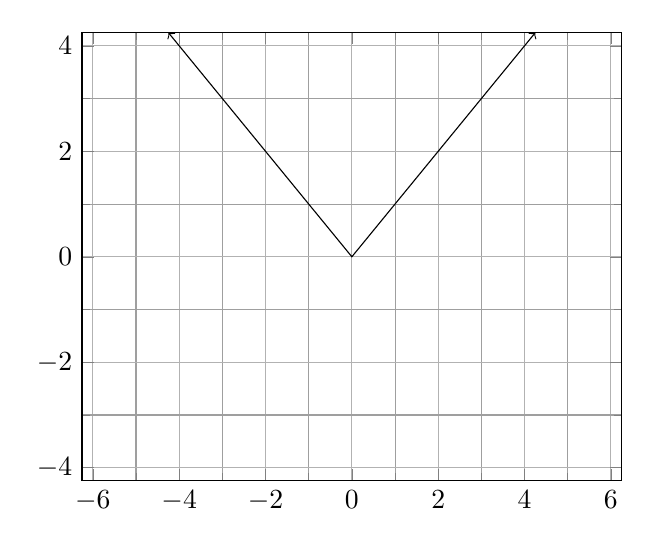
\begin{tikzpicture}[declare function={
          f(\x)=abs(\x);}]
          \begin{axis}[
            grid=both, %major,minor
            grid style={line width=0.375pt, draw=gray!60},
            minor grid style={draw=gray!75},
            xmin=-6.25, xmax=6.25,
            ymin=-4.25, ymax=4.25,
            minor x tick num=1,
            minor y tick num=1,
            ]
            \addplot[<->] expression[domain=-4.25:4.25]{f(x)};
          \end{axis}
        \end{tikzpicture}
    \end{extasks}
  \end{ex*}
  \pagebreak

  %Even and odd functions
  \begin{defn*}[Even and Odd functions]
    A function is called an even function if for every input $x$
      \[f(x)=f(-x)\]
    The graph of an even function is symmetric about the $y-$axis.
    \vspace*{0.5\baselineskip}

    A function is called an odd function if for every input $x$
      \[f(x)=-f(-x)\]
    The graph of an odd function is symmetric about the origin.
  \end{defn*}

  \begin{ex*}
    Using algebra, determine if the following functions are even, odd, or neither:
    \hspace*{\stretch{1}}
    \textcolor{blue}{\underline{\href{https://www.desmos.com/calculator/jezmca9ufn}{Graphs}}}
    \begin{extasks}[after-item-skip=\stretch{1}](2)
      \task $f(x)=x^3$
      \task $g(x)=\abs{x}+1$
      \task $h(x)=(x-1)^2$
      \task $j(x)=x^3-\dfrac{1}{x}$
    \end{extasks}
    \vspace*{\stretch{1}}
  \end{ex*}
  \pagebreak

  %Stretches and compressions
  \begin{defn*}[Vertical Stretches and Compressions]
    Given a function $f(x)$, a new function $g(x)=af(x)$, where $a$ is a constant, is a \textbf{vertical stretch} or \textbf{vertical compression} of the function $f(x)$.
    \begin{itemize}
      \item If $a>1$, then the graph will be stretched.
      \item If $0<a<1$, then the graph will be compressed.
      \item If $a<0$, then there will be a combination of a vertical stretch/compression with a vertical reflection.
    \end{itemize}
  \end{defn*}

  \begin{ex*}
    Given the graph of $f(x)$ below, graph $g(x)=2f(x)$:
    \hspace*{\stretch{1}}
    \textcolor{blue}{\underline{\href{https://www.desmos.com/calculator/7khrjmegyi}{Graphs}}}
    \begin{center}
      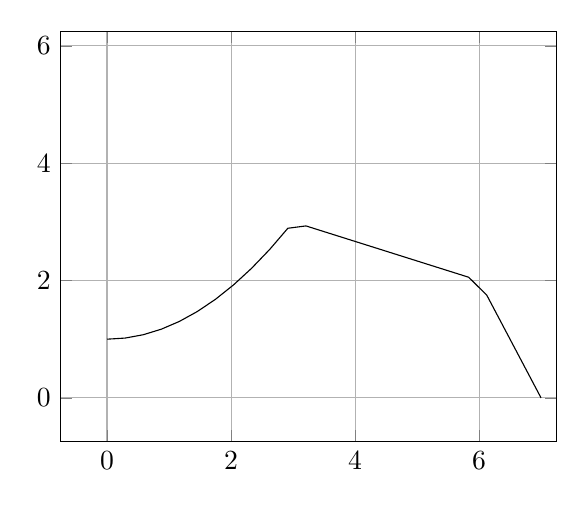
\begin{tikzpicture}[declare function={
        f(\x)=\x<=3 ? 2*\x^2/9+1 :
              (\x<=6 ? -\x/3 + 4  : 14-2*\x);
        }]
        \begin{axis}[
            grid=both, %major,minor
            grid style={line width=0.375pt, draw=gray!60},
            minor grid style={draw=gray!75},
            xmin=-0.75, xmax=7.25,
            ymin=-0.75, ymax=6.25,
            width=0.65*\linewidth,
            ]
            \addplot[-] expression[domain=0:7]{f(x)};
        \end{axis}
      \end{tikzpicture}
    \end{center}
  \end{ex*}
  \pagebreak

  \begin{defn*}[Horizontal Stretches and Compressions]
    Given a function $f(x)$, a new function $g(x)=f(bx)$, where $b$ is a constant, is a \textbf{horizontal stretch} or \textbf{horizontal compression} of the function $f(x)$.
    \begin{itemize}
      \item If $b>1$, then the graph will be stretched by $\dfrac{1}{b}$.
      \item If $0<b<1$, then the graph will be compressed by $\dfrac{1}{b}$.
      \item If $b<0$, then there will be a combination of a horizontal stretch/compression with a horizontal reflection.
    \end{itemize}
  \end{defn*}

  \begin{ex*}
    Given the graph of $f(x)$ below, graph $g(x)=f(2x)$:
    \hspace*{\stretch{1}}
    \textcolor{blue}{\underline{\href{https://www.desmos.com/calculator/7khrjmegyi}{Graphs}}}
    \begin{center}
      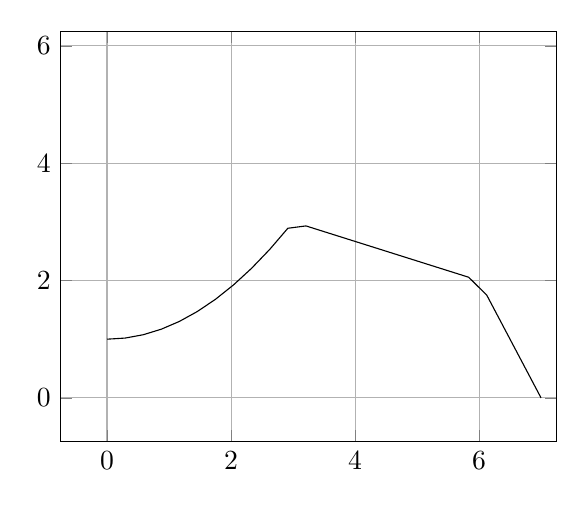
\begin{tikzpicture}[declare function={
        f(\x)=\x<=3 ? 2*\x^2/9+1 :
              (\x<=6 ? -\x/3 + 4  : 14-2*\x);
        }]
        \begin{axis}[
            grid=both, %major,minor
            grid style={line width=0.375pt, draw=gray!60},
            minor grid style={draw=gray!75},
            xmin=-0.75, xmax=7.25,
            ymin=-0.75, ymax=6.25,
            width=0.65*\linewidth,
            ]
            \addplot[-] expression[domain=0:7]{f(x)};
        \end{axis}
      \end{tikzpicture}
    \end{center}
  \end{ex*}
  \pagebreak

  % sequence of transformations
  \TabPositions{30mm}
  \begin{thmBox*}[Combining Transformations]
    When combining transformations \dots
    \begin{itemize}
      \item
        $af(x)+k$: \tab first vertically stretch by $a$ and then shift by $k$.
      \item
        $f(bx-h)$: \tab first horizontally shift by $h$ and then horizontally stretch by $\dfrac{1}{b}$.
      \item
        $f(b(x-h))$: \tab first horizontally stretch by $\dfrac{1}{b}$ and then horizontally shift by $h$.
      \item
        Horizontal and vertical transformations are independent of the order them are performed.
    \end{itemize}
  \end{thmBox*}

  \begin{ex*}
    Given the graph of $f(x)$ below, graph $g(x)=f\parens{\dfrac{1}{2}x+1}-3$:
    \hspace*{\stretch{1}}
    \textcolor{blue}{\underline{\href{https://www.desmos.com/calculator/orwapzvycw}{Graphs}}}
    \begin{center}
      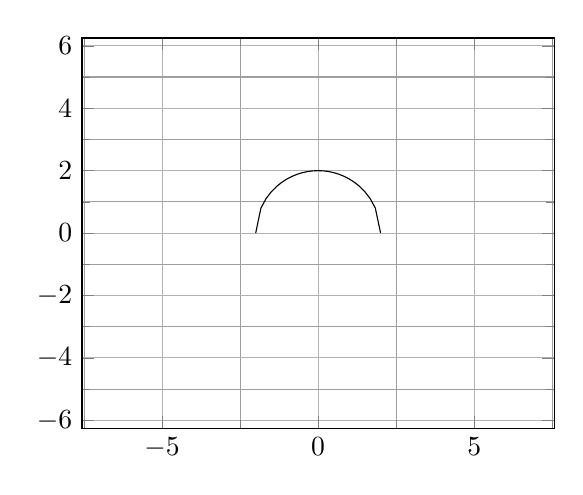
\begin{tikzpicture}[declare function={
        f(\x)=sqrt(4-x^2);
        }]
        \begin{axis}[
            grid=both, %major,minor
            grid style={line width=0.375pt, draw=gray!60},
            axis equal,
            minor grid style={draw=gray!75},
            ymin=-6.25, ymax=6.25,
            width=0.625*\linewidth,
            minor x tick num=1,
            minor y tick num=1,
            ]
            \addplot[-] expression[domain=-2:2]{f(x)};
        \end{axis}
      \end{tikzpicture}
    \end{center}
  \end{ex*}
  \pagebreak

  %TODO pick out homework problems

  \pagebreak
\end{document}
